The N-Queens puzzle is the problem of placing N chess queens on an NxN
chessboard so that no pair of two queens attack each
other~\cite{8queens}. The challenge of finding all the
distinct solutions to this problem is a good benchmark in designing
parallel algorithms.

The LM solution considers the chess board as a graph where nodes communicate
with each other to build valid configurations. First, we start with the empty
state in the first row of the chess board. Then, each square adds its own
position to the state and sends the state down, to the next row. Once a square
receives new configurations, it attempts to add its position to the
configurations. If valid, that configuration is then sent, recursively, to the
next row, until all rows are traversed. At the end of the program, the nodes at
the bottom row will have all the valid configurations.

Since computation goes from the top row to the bottom row, not all placements of
nodes on threads may be equally performant. This is specially true because the
bottom rows tend to perform most work. The best placement is then to split the
board vertically, so that, in optimal conditions, each thread gets the same
number of columns.  Our experiments show that, on shared memory, it does not
matter much if we start with a bad placement since node stealing overcomes those
issues by improving load balancing dynamically. But what if we want run the
program on a distributed system, where moving nodes between workers can be
expensive? We measured the performance of the program without node stealing in
order to assess how important data placement would be for such systems.
We used the default partition of the program as it is, which results in the board being
split by rows and another configuration using the coordination action
\texttt{set-cpu(A, vertical(X, Y))} that forces nodes to be moved to another
thread using a vertical partitioning. Note that \texttt{X} and \texttt{Y} are
the coordinates of the node in the chessboard.

Figure~\ref{results:nqueens} shows the performance results of coordinating the
placing of nodes on threads without work stealing. There is a noticiable
performance improvement when using an optimal data placement strategy. Note
however that in the plot we do not take into account the costs of moving
nodes between workers. In a real system, the performance gap may not be as wide
since in the worst case there may be 144 moves.

\begin{figure}[ht!]
   \begin{center}
      \subfloat[]{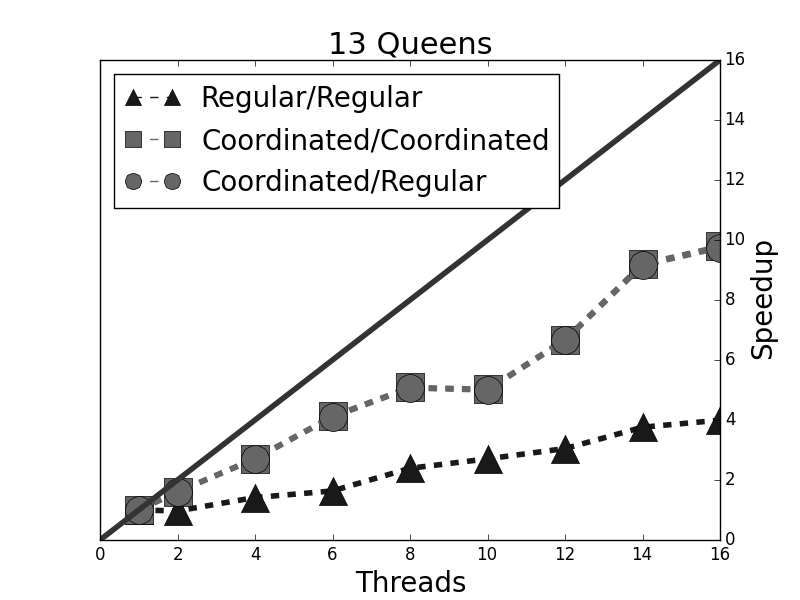
\includegraphics[width=5cm]{results/13queens.png}}
   \end{center}
   \caption{Experimental results for the 13 Queens program. The coordinated
      version is on average 2 times faster than the version with bad data
      placement.}
   \label{results:nqueens}
\end{figure}
